% Metódy inžinierskej práce

\documentclass[10pt,twoside,slovak,a4paper]{article}

\usepackage[slovak]{babel}
%\usepackage[T1]{fontenc}
\usepackage[IL2]{fontenc} % lepšia sadzba písmena Ľ než v T1
\usepackage[utf8]{inputenc}
\usepackage{graphicx}
\usepackage{url} % príkaz \url na formátovanie URL
\usepackage{hyperref} % odkazy v texte budú aktívne (pri niektorých triedach dokumentov spôsobuje posun textu)

\usepackage{cite}
%\usepackage{times}

\pagestyle{headings}

\title{Využitie umelej inteligencie a GPT na získavanie a spracovanie informácií v
oblasti vzdelávania\thanks{Semestrálny projekt v predmete Metódy inžinierskej práce, ak. rok 2023/24, vedenie: Mgr. Martin Sabo, Phd.}} % meno a priezvisko vyučujúceho na cvičeniach

\author{Bálint Janik\\[2pt]
	{\small Slovenská technická univerzita v Bratislave}\\
	{\small Fakulta informatiky a informačných technológií}\\
	{\small \texttt{xjanikb@stuba.sk}}
	}

\date{\small 30. september 2023} % upravte



\begin{document}

\maketitle

\begin{abstract}
Umelá inteligencia postupne prechádza revolučnými zmenami, ktoré umožňujú vývoj ChatBotov, ktoré nielenže vytvárajú dojem písania si s reálnou osobou, ale sú výbornými zdrojmi informácií využívanými najmä v oblasti vzdelávania. Generatívny predtrénovaný transformátor (GPT), na ktorom firma OpenAI postavila svoj chatbot ChatGPT vykazuje mimoriadne vysoké výsledky a presnosť, čo dokazuje aj jej schopnosť vyriešiť množstvo náročných skúšok. Po jej boku sa rovnako vyvíja so sofistikovanejším obsahom generatívna umelá inteligencia (GAI), ktorá je schopná na základe hlbokého učenia, využívania dostupných knižníc údajov a analýzy poskytnutých údajov sprevádzať vzdelávanie. Aj keď má umelá inteligencia mohutný dopad na všetky oblasti vzdelávania, niektorí upozorňujú na riziká spojené s jej využívaním. Cieľom tohto článku je priblížiť funkciu umelej inteligencie, jej spôsobu práce s údajmi, ako aj jeho využitie v oblasti vzdelávania.
\end{abstract}



\section{Úvod}

Motivujte čitateľa a vysvetlite, o čom píšete. Úvod sa väčšinou nedelí na časti.

Uveďte explicitne štruktúru článku. Tu je nejaký príklad.
Základný problém, ktorý bol naznačený v úvode, je podrobnejšie vysvetlený v časti~\ref{nejaka}.
Dôležité súvislosti sú uvedené v častiach~\ref{dolezita} a~\ref{dolezitejsia}.
Záverečné poznámky prináša časť~\ref{zaver}.



\section{Nejaká časť} \label{nejaka}

Z obr.~\ref{f:rozhod} je všetko jasné. 

\begin{figure*}[tbh]
\centering
%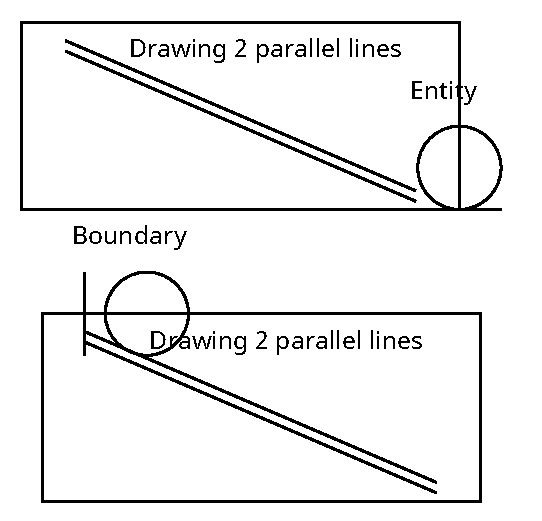
\includegraphics[scale=1.0]{diagram.pdf}
Aj text môže byť prezentovaný ako obrázok. Stane sa z neho označný plávajúci objekt. Po vytvorení diagramu zrušte znak \texttt{\%} pred príkazom \verb|\includegraphics| označte tento riadok ako komentár (tiež pomocou znaku \texttt{\%}).
\caption{Rozhodujúci argument.}
\label{f:rozhod}
\end{figure*}



\section{Iná časť} \label{ina}

Základným problémom je teda\ldots{} Najprv sa pozrieme na nejaké vysvetlenie (časť~\ref{ina:nejake}), a potom na ešte nejaké (časť~\ref{ina:nejake}).\footnote{Niekedy môžete potrebovať aj poznámku pod čiarou.}

Môže sa zdať, že problém vlastne nejestvuje\cite{Coplien:MPD}, ale bolo dokázané, že to tak nie je~\cite{Czarnecki:Staged, Czarnecki:Progress}. Napriek tomu, aj dnes na webe narazíme na všelijaké pochybné názory\cite{starting-article}. Dôležité veci možno \emph{zdôrazniť kurzívou}.


\subsection{Nejaké vysvetlenie} \label{ina:nejake}

Niekedy treba uviesť zoznam:

\begin{itemize}
\item jedna vec
\item druhá vec
	\begin{itemize}
	\item x
	\item y
	\end{itemize}
\end{itemize}

Ten istý zoznam, len číslovaný:

\begin{enumerate}
\item jedna vec
\item druhá vec
	\begin{enumerate}
	\item x
	\item y
	\end{enumerate}
\end{enumerate}


\subsection{Ešte nejaké vysvetlenie} \label{ina:este}

\paragraph{Veľmi dôležitá poznámka.}
Niekedy je potrebné nadpisom označiť odsek. Text pokračuje hneď za nadpisom.



\section{Dôležitá časť} \label{dolezita}
\paragraph{Lorem ipsum dolor sit amet, consectetur adipiscing elit, sed do eiusmod tempor incididunt ut labore et dolore magna aliqua. Ut enim ad minim veniam, quis nostrud exercitation ullamco laboris nisi ut aliquip ex ea commodo consequat. Duis aute irure dolor in reprehenderit in voluptate velit esse cillum dolore eu fugiat nulla pariatur. Excepteur sint occaecat cupidatat non proident, sunt in culpa qui officia deserunt mollit anim id est laborum.}

\paragraph{Lorem ipsum dolor sit amet, consectetur adipiscing elit, sed do eiusmod tempor incididunt ut labore et dolore magna aliqua. Ut enim ad minim veniam, quis nostrud exercitation ullamco laboris nisi ut aliquip ex ea commodo consequat. Duis aute irure dolor in reprehenderit in voluptate velit esse cillum dolore eu fugiat nulla pariatur. Excepteur sint occaecat cupidatat non proident, sunt in culpa qui officia deserunt mollit anim id est laborum.}




\section{Ešte dôležitejšia časť} \label{dolezitejsia}
\paragraph{Lorem ipsum dolor sit amet, consectetur adipiscing elit, sed do eiusmod tempor incididunt ut labore et dolore magna aliqua. Ut enim ad minim veniam, quis nostrud exercitation ullamco laboris nisi ut aliquip ex ea commodo consequat. Duis aute irure dolor in reprehenderit in voluptate velit esse cillum dolore eu fugiat nulla pariatur. Excepteur sint occaecat cupidatat non proident, sunt in culpa qui officia deserunt mollit anim id est laborum.}



\section{Zhodnotenie} \label{zaver} % prípadne iný variant názvu
\paragraph{Lorem ipsum dolor sit amet, consectetur adipiscing elit, sed do eiusmod tempor incididunt ut labore et dolore magna aliqua. Ut enim ad minim veniam, quis nostrud exercitation ullamco laboris nisi ut aliquip ex ea commodo consequat. Duis aute irure dolor in reprehenderit in voluptate velit esse cillum dolore eu fugiat nulla pariatur. Excepteur sint occaecat cupidatat non proident, sunt in culpa qui officia deserunt mollit anim id est laborum.}


\paragraph{Lorem ipsum dolor sit amet, consectetur adipiscing elit, sed do eiusmod tempor incididunt ut labore et dolore magna aliqua. Non nisi est sit amet facilisis. Aliquet risus feugiat in ante metus dictum at. Eget velit aliquet sagittis id consectetur. Eleifend mi in nulla posuere sollicitudin aliquam ultrices sagittis orci. Magna fringilla urna porttitor rhoncus dolor purus. Ultrices sagittis orci a scelerisque purus. Non tellus orci ac auctor augue mauris augue. Pretium nibh ipsum consequat nisl vel pretium lectus. Eros donec ac odio tempor orci dapibus ultrices in iaculis. Elit ut aliquam purus sit. Sed elementum tempus egestas sed sed risus pretium quam vulputate. Orci eu lobortis elementum nibh tellus molestie nunc non. Sagittis id consectetur purus ut faucibus pulvinar elementum integer. Vitae ultricies leo integer malesuada nunc vel risus. Adipiscing bibendum est ultricies integer quis auctor elit. Ut pharetra sit amet aliquam id}





\section{Záver} \label{mojaskt}
\paragraph{Lorem ipsum dolor sit amet, consectetur adipiscing elit, sed do eiusmod tempor incididunt ut labore et dolore magna aliqua. Ut enim ad minim veniam, quis nostrud exercitation ullamco laboris nisi ut aliquip ex ea commodo consequat. Duis aute irure dolor in reprehenderit in voluptate velit esse cillum dolore eu fugiat nulla pariatur. Excepteur sint occaecat cupidatat non proident, sunt in culpa qui officia deserunt mollit anim id est laborum.}

%\acknowledgement{Ak niekomu chcete poďakovať\ldots}

% týmto sa generuje zoznam literatúry z obsahu súboru literatura.bib podľa toho, na čo sa v článku odkazujete
\bibliography{literatura}
\bibliographystyle{abbrv} % prípadne alpha, abbrv alebo hociktorý iný



\end{document}